%%%%%%%%%%%%%%%%%%%%%%%%%%%%%%%%%%%%%%%%%
% NIH Grant Proposal for the Specific Aims and Research Plan Sections
% LaTeX Template
% Version 1.0 (21/10/13)
%
% This template has been downloaded from:
% http://www.LaTeXTemplates.com
%
% Original author:
% Erick Tatro (erickttr@gmail.com) with modifications by:
% Vel (vel@latextemplates.com)
%
% Adapted from:
% J. Hrabe (http://www.magalien.com/public/nih_grants_in_latex.html)
%
% License:
% CC BY-NC-SA 3.0 (http://creativecommons.org/licenses/by-nc-sa/3.0/)
%
%%%%%%%%%%%%%%%%%%%%%%%%%%%%%%%%%%%%%%%%%

%----------------------------------------------------------------------------------------
%	PACKAGES AND OTHER DOCUMENT CONFIGURATIONS
%----------------------------------------------------------------------------------------

\documentclass[11pt,notitlepage]{article}

% A note on fonts: As of 2013, NIH allows Georgia, Arial, Helvetica, and Palatino Linotype. LaTeX doesn't have Georgia or Arial built in; you can try to come up with your own solution if you wish to use those fonts. Here, Palatino & Helvetica are available, leave the font you want to use uncommented while commenting out the other one.
\usepackage{palatino} % Palatino font
%\usepackage{helvet} % Helvetica font
\renewcommand*\familydefault{\sfdefault} % Use the sans serif version of the font
\usepackage[T1]{fontenc}
\linespread{1.05} % A little extra line spread is better for the Palatino font

\usepackage{lipsum} % Used for inserting dummy 'Lorem ipsum' text into the template
\usepackage{amsfonts, amsmath, amsthm, amssymb} % For math fonts, symbols and environments
\usepackage{graphicx} % Required for including images
\usepackage{booktabs} % Top and bottom rules for table
\usepackage{wrapfig} % Allows in-line images
\usepackage[labelfont=bf]{caption} % Make figure numbering in captions bold
\usepackage[top=0.5in,bottom=0.5in,left=0.5in,right=0.5in]{geometry} % Reduce the size of the margin
\pagestyle{empty} % Remove page numbers

\hyphenation{ionto-pho-re-tic iso-tro-pic fortran} % Specifies custom hyphenation points for words or words that shouldn't be hyphenated at all

\begin{document}

%----------------------------------------------------------------------------------------
%	SPECIFIC AIMS
%----------------------------------------------------------------------------------------

\section*{Specific Aims}

This is an example citation \cite{Tatro2013}. \lipsum[1-3]

\begin{description}

\item[Aim 1: Really cool stuff.]{}
\item{1.1. First sub-aim with more details}
\item{1.2. Second sub-aim with more details.}
\end{description}

\begin{description}
\item[Aim 2: Really cool stuff.]{}
\item{2.1. First sub-aim with more details.}
\item{2.2. Second sub-aim with more details.}
\end{description}

\begin{description}
\item[Aim 3: Really cool stuff.]{ }
\item{3.1. First sub-aim with more details.}
\item {3.2. Second sub-aim with more details.}
\item{3.3. Third sub-aim with more details.}
\end{description}

\lipsum[100]

\newpage
%=======INSTRUCTIONS FOR SIGNIFICANCE==========

\section*{A. Significance}

\begin{description} % For subheadings within a section, this template uses the {description} environment, it is not obtrusively large like a \subsection; and facilitates a brief optional subtitle; and it will wrap around figures and tables; it also has a decent amount of whitespace above/below which is less than for a section heading
\item[A.1. Instructions.]{Optional subtitle}
\end{description}

Explain the importance of the problem or critical barrier to progress in the field that the proposed project addresses.

Explain how the proposed project will improve scientific knowledge, technical capability, and/or clinical practice in one or more broad fields.

Describe how the concepts, methods, technologies, treatments, services, or preventative interventions that drive this field will be changed if the proposed aims are achieved.

\begin{description}
\item[A.2. Subheading.]{}
\end{description}

\begin{wraptable}{r}{4.8cm} % Example table with text wrapping around it
\caption{Example Table}
\begin{center}
\begin{tabular}{l l r}
\toprule
\multicolumn{1}{c}{City} & {N\textsuperscript{a}} & {\%Silly}\\
\midrule
San Diego & 289 & 41\%\\
Seattle & 262 & 32\%\\
Galveston & 261 & 15\%\\
St Louis & 269 & 7\%\\
New York & 271 & 4\%\\
Baltimore & 231 & 2\%\\
\emph{Total} & 1,586 & 21\%\\
\hline
\end{tabular}\\
\footnotesize\textsuperscript{a}{All participants clowns.}
\end{center}
\label{default}
\end{wraptable}

\lipsum[8-10]

\begin{wrapfigure}{r}{6.8cm} % Example figure with text wrapping around it
\includegraphics[scale=0.9]{Figures/Fig1.pdf}
\caption{\footnotesize Example wrapped figure. (A) Impressive microscopy image. (B) Impressive data.}
\end{wrapfigure}

\lipsum[5]

\begin{description}
\item[A.3. Another subheading:]{optional subtitle.}
\end{description}

\lipsum[25]

\begin{figure}[b] % Centered big figure at bottom of the page ([b] argument, could be "t" for top or "h" for here)
\centering
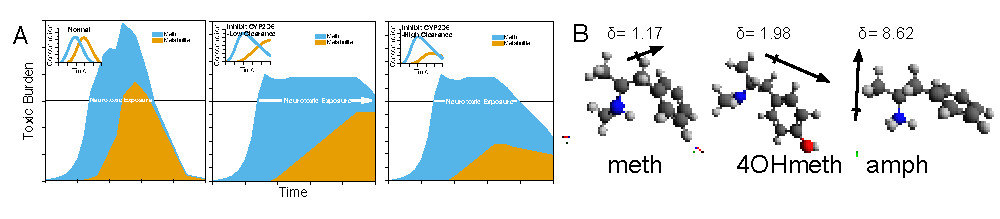
\includegraphics[scale = .80]{Figures/Fig2.pdf}
\caption{\footnotesize Big Figure legend Big Figure legend Big Figure legend Big Figure legend Big Figure legend Big Figure legend Big Figure legend Big Figure legend Big Figure legend.}
\label{fig2}
\end{figure}

\lipsum[31-32]

\begin{description}
\item[A.4. Yet another subheading.]{}
\end{description}

\lipsum[55-56]

%========INSTRUCTIONS FOR INNOVATION================

\section*{B. Innovation}

\begin{description}
\item[B.1. Instructions.]{}
\end{description}

Explain how the application challenges and seeks to shift current research or clinical practice paradigms.

Describe any novel theoretical concepts, approaches or methodologies, instrumentation or interventions to be developed or used, and any advantage over existing methodologies, instrumentation, or interventions.

Explain any refinements, improvements, or new applications of theoretical concepts, approaches or methodologies, instrumentation, or interventions.

%========INSTRUCTIONS FOR APPROACH================

\section*{C. Approach}

\begin{description}
\item[C.1. Instructions.]{}
\end{description}

Describe the overall strategy, methodology, and analyses to be used to accomplish the specific aims of the project. Unless addressed separately in Item 15 (Resource Sharing Plan), include how the data will be collected, analyzed, and interpreted as well as any resource sharing plans as appropriate.

Discuss potential problems, alternative strategies, and benchmarks for success anticipated to achieve the aims.

If the project is in the early stages of development, describe any strategy to establish feasibility, and address the management of any high risk aspects of the proposed work.

Point out any procedures, situations, or materials that may be hazardous to personnel and precautions to be exercised. A full discussion on the use of Select Agents should appear in Item 11, below.

As applicable, also include the following information as part of the Research Strategy, keeping within the three sections listed above: Significance, Innovation, and Approach.

\begin{description}
\item[C.2. Preliminary Studies for New Applications]{}
\end{description}

Preliminary Studies for New Applications: For new applications, include information on Preliminary Studies. Discuss the PD/PI's preliminary studies, data, and or experience pertinent to this application. Except for Exploratory/Developmental Grants (R21/R33), Small Research Grants (R03), and Academic Research Enhancement Award (AREA) Grants (R15), preliminary data can be an essential part of a research grant application and help to establish the likelihood of success of the proposed project. Early Stage Investigators should include preliminary data (however, for R01 applications, reviewers will be instructed to place less emphasis on the preliminary data in application from Early Stage Investigators than on the preliminary data in applications from more established investigators).

%------------------------------------------------

%----------------------------------------------------------------------------------------
%	RESEARCH PLAN
%----------------------------------------------------------------------------------------

% \newpage

% \section*{5. Progress Report Publication List (Renewal Applications Only)}

% List the titles and complete references to all appropriate publications, manuscripts accepted for publication, patents, and other printed materials that have resulted from the project since it was last reviewed competitively. When citing articles that fall under the Public Access Policy, were authored or co-authored by the applicant and arose from NIH support, provide the NIH Manuscript Submission reference number (e.g., NIHMS97531) or the Pubmed Central (PMC) reference number (e.g., PMCID234567) for each article. If the PMCID is not yet available because the Journal submits articles directly to PMC on behalf of their authors, indicate "PMC Journal -- In Process." A list of these journals is posted at: http://publicaccess.nih.gov/submit\_process\_journals.htm.

% Citations that are not covered by the Public Access Policy, but are publicly available in a free, online format may include URLs or PMCID numbers along with the full reference (note that copies of these publications are not accepted as appendix material, see Part I Section 5.5.15 for more information).

%------------------------------------------------

\newpage

\section*{6. Protection of Human Subjects}

Refer to Part II, Supplemental Instructions for Preparing the Human Subjects Section of the Research Plan.

This section is required for applicants answering "yes" to the question "Are human subjects involved?" on the R\&R Other Project Information form. If the answer is "No" to the question but the proposed research involves human specimens and/or data from subjects applicants must provide a justification in this section for the claim that no human subjects are involved.

Do not use the protection of human subjects section to circumvent the page limits of the Research Strategy.

%------------------------------------------------

\newpage

\section*{7. Inclusion of Women and Minorities}

Refer to Part II, Supplemental Instructions for Preparing the Human Subjects Section of the Research Plan. This section is required for applicants answering "yes" to the question "Are human subjects involved?" on the R\&R Other Project Information form and the research does not fall under Exemption 4.

%------------------------------------------------

\newpage

%   \section*{8. Targeted/Planned Enrollment} - form to fill out
\section*{9. Inclusion of Children}

Refer to Supplemental Instructions for Preparing the Human Subjects Section of the Research Plan, Sections 4.4 and 5.7. For applicants answering "Yes" to the question "Are human subjects involved" on the R\&R Other Project Information Form and the research does not fall under Section 4, this section is required.

%------------------------------------------------

\newpage

\section*{10. Vertebrate Animals}

If Vertebrate Animals are involved in the project, address each of the five points below. This section should be a concise, complete description of the animals and proposed procedures. While additional details may be included in the Research Strategy, the responses to the five required points below must be cohesive and include sufficient detail to allow evaluation by peer reviewers and NIH staff. If all or part of the proposed research involving vertebrate animals will take place at alternate sites (such as project/performance or collaborating site(s)), identify those sites and describe the activities at those locations. Although no specific page limitation applies to this section of the application, be succinct. Failure to address the following five points will result in the application being designated as incomplete and will be grounds for the PHS to defer the application from the peer review round. Alternatively, the application’s impact/priority score may be negatively affected.

If the involvement of animals is indefinite, provide an explanation and indicate when it is anticipated that animals will be used. If an award is made, prior to the involvement of animals the grantee must submit to the NIH awarding office detailed information as required in points 1-5 above and verification of IACUC approval. If the grantee does not have an Animal Welfare Assurance then an appropriate Assurance will be required (See Part III, Section 2.2 Vertebrate Animals for more information).
The five points are as follows:

\begin{enumerate}
\item Provide a detailed description of the proposed use of the animals in the work outlined in the Research Strategy section. Identify the species, strains, ages, sex, and numbers of animals to be used in the proposed work.
\item Justify the use of animals, the choice of species, and the numbers to be used. If animals are in short supply, costly, or to be used in large numbers, provide an additional rationale for their selection and numbers.
\item Provide information on the veterinary care of the animals involved.
\item Describe the procedures for ensuring that discomfort, distress, pain, and injury will be limited to that which is unavoidable in the conduct of scientifically sound research. Describe the use of analgesic, anesthetic, and tranquilizing drugs and/or comfortable restraining devices, where appropriate, to minimize discomfort, distress, pain, and injury.
\item Describe any method of euthanasia to be used and the reasons for its selection. State whether this method is consistent with the recommendations of the American Veterinary Medical Association (AVMA) Guidelines on Euthanasia. If not, include a scientific justification for not following the recommendations.
\end{enumerate}

Do not use the vertebrate animal section to circumvent the page limits of the Research Strategy.

%------------------------------------------------

\newpage

\section*{11. Select Agent Research}

Select Agents are hazardous biological agents and toxins that have been identified by DHHS or USDA as having the potential to pose a severe threat to public health and safety, to animal and plant health, or to animal and plant products. CDC maintains a list of these agents. See http://www.cdc.gov/od/sap/docs/salist.pdf.

%------------------------------------------------

\newpage

\section*{12. Multiple PD/PI Leadership Plan}

For applications designating multiple PD/PIs, a leadership plan must be included. A rationale for choosing a multiple PD/PI approach should be described. The governance and organizational structure of the leadership team and the research project should be described, including communication plans, process for making decisions on scientific direction, and procedures for resolving conflicts. The roles and administrative, technical, and scientific responsibilities for the project or program should be delineated for the PD/PIs and other collaborators.

If budget allocation is planned, the distribution of resources to specific components of the project or the individual PD/PIs should be delineated in the Leadership Plan. In the event of an award, the requested allocations may be reflected in a footnote on the Notice of Grant Award.

%------------------------------------------------

\newpage

\section*{13. Consortium/Contractual Arrangements}

Explain the programmatic, fiscal, and administrative arrangements to be made between the applicant organization and the consortium organization(s). If consortium/contractual activities represent a significant portion of the overall project, explain why the applicant organization, rather than the ultimate performer of the activities, should be the grantee. The signature of the Authorized Organization Representative on the SF424 (R\&R) cover component (Item 17) signifies that the applicant and all proposed consortium participants understand and agree to the following statement:

\emph{The appropriate programmatic and administrative personnel of each organization involved in this grant application are aware of the agency's consortium agreement policy and are prepared to establish the necessary inter-organizational agreement(s) consistent with that policy.}

%------------------------------------------------

\newpage

%   \section*{14. Letters of Support} - letters to attach
\section*{15. Resource Sharing}

NIH considers the sharing of unique research resources developed through NIH-sponsored research an important means to enhance the value and further the advancement of the research. When resources have been developed with NIH funds and the associated research findings published or provided to NIH, it is important that they be made readily available for research purposes to qualified individuals within the scientific community. See Part III, 1.5 Sharing Research Resources.

\begin{enumerate}
\item{Data Sharing Plan:} Investigators seeking \$500,000 or more in direct costs (exclusive of consortium F\&A) in any year are expected to include a brief 1-paragraph description of how final research data will be shared, or explain why data-sharing is not possible. Specific Funding Opportunity Announcements may require that all applications include this information regardless of the dollar level. Applicants are encouraged to read the specific opportunity carefully and discuss their data-sharing plan with their program contact at the time they negotiate an agreement with the Institute/Center (IC) staff to accept assignment of their application. See Data-Sharing Policy or http://grants.nih.gov/grants/guide/notice- files/NOT-OD-03-032.html.
\item{Sharing Model Organisms:} Regardless of the amount requested, all applications where the development of model organisms is anticipated are expected to include a description of a specific plan for sharing and distributing unique model organisms or state why such sharing is restricted or not possible. See Sharing Model Organisms Policy, and NIH Guide NOT-OD-04-042.
\item{Genome Wide Association Studies (GWAS):} Applicants seeking funding for a genome-wide association study are expected to provide a plan for submission of GWAS data to the NIH-designated GWAS data repository, or an appropriate explanation why submission to the repository is not possible. GWAS is defined as any study of genetic variation across the entire genome that is designed to identify genetic associations with observable traits (such as blood pressure or weight) or the presence or absence of a disease or condition. For further information see Policy for Sharing of Data Obtained in NIH Supported or Conducted Genome-Wide Association Studies, NIH Guide NOT-OD-07-088, and http://grants.nih.gov/grants/gwas/.
\end{enumerate}

%----------------------------------------------------------------------------------------
%	BIBLIOGRAPHY
%----------------------------------------------------------------------------------------

\newpage

\bibliography{proposal} % Use the NIHGrant.bib file for the reference list
\bibliographystyle{nihunsrt} % Use the custom nihunsrt bibliography style included with the template

%----------------------------------------------------------------------------------------

\end{document}